%\documentstyle[epsf,twocolumn]{jarticle}       %LaTeX2e仕様
\documentclass[twocolumn]{jarticle}     %pLaTeX2e仕様(platex.exeの場合)
%\documentclass[twocolumn]{ujarticle}     %pLaTeX2e仕様(uplatex.exeの場合)
%%%%%%%%%%%%%%%%%%%%%%%%%%%%%%%%%%%%%%%%%%%%%%%%%%%%%%%%%%%%%%
%%
%%  基本バージョン
%%
%%%%%%%%%%%%%%%%%%%%%%%%%%%%%%%%%%%%%%%%%%%%%%%%%%%%%%%%%%%%%%%%
\setlength{\topmargin}{-45pt}
%\setlength{\oddsidemargin}{0cm} 
\setlength{\oddsidemargin}{-7.5mm}
%\setlength{\evensidemargin}{0cm} 
\setlength{\textheight}{24.1cm}
%setlength{\textheight}{25cm} 
\setlength{\textwidth}{17.4cm}
%\setlength{\textwidth}{172mm} 
\setlength{\columnsep}{11mm}

\kanjiskip=.07zw plus.5pt minus.5pt


% 【節が変わるごとに (1.1)(1.2) … (2.1)(2.2) と数式番号をつけるとき】
%\makeatletter
%\renewcommand{\theequation}{%
%\thesection.\arabic{equation}} %\@addtoreset{equation}{section}
%\makeatother

%\renewcommand{\arraystretch}{0.95} 行間の設定

%%%%%%%%%%%%%%%%%%%%%%%%%%%%%%%%%%%%%%%%%%%%%%%%%%%%%%%%
\usepackage[dvipdfmx]{graphicx}   %pLaTeX2e仕様(\documentstyle ->\documentclass)\documentclass[dvipdfmx]{graphicx}
\usepackage[subrefformat=parens]{subcaption}
%%%%%%%%%%%%%%%%%%%%%%%%%%%%%%%%%%%%%%%%%%%%%%%%%%%%%%%%

\begin{document}

\twocolumn[
\noindent

\hspace{1em}
\today
\hfill
\ \ 細川 岳大

\vspace{2mm}

\hrule

\begin{center}
{\Large \bf 進捗報告}
\end{center}
\hrule
\vspace{3mm}
]

% ‚ここから 文章 Start!
\section{今週やったこと}
 GAを用いたDataAugmentaion

\section{実験}
前回に引き続きGAを用いたDataAugmentationの実験を行った.

\subsection{実験データ}
実験データはcifar10を用いて,
事前学習ではepoch数300,train\_dataを各ラベル5000枚の計50000枚使用し,GAで学習する際はepoch数100,train\_dataは各ラベル200枚のオリジナルとそれらすべてをDataAugmentaionしたものとを合わせ計4000枚とし,test\_dataは共に10000枚とした.また事前学習でのaccuracyは0.8475である.
\subsection{遺伝的アルゴリズム}


\subsubsection{探索空間}
\ 探索する水増し操作として画素値操作(Sharpness,Posterize,Brightness,Autoconstrast,Equalize,Solarize,Invert,Contrast,ColorBalance),
変形操作(Mirror,Translate X/Y,Shear X/Y,Rotate)の15種類の操作であり,今回はそれらすべてを個別にどの程度強くかけるかおよびどの順序でかけるかということを探索する.各操作についての強度の最大最小を設定し,それを0\%から100\%まで25\%ずつ分け5段階の度合いとする.ただし,Autocontrast,Equalize,Invert,Mirror については適用するか否かであるためパラメータが3以上で適用するとした.強度は0から5の整数値を持つ15個の遺伝子を実数値コーディングによって表現する.
また,適用順序に関しては同様に15個の遺伝子を持つ順列コーディングによって表現する.つまり,探索空間は$2^4*5^{11}*15!=10^{21}$となる.

\subsubsection{選択}
\ 選択について,エリート選出によって最も適応度の高い2つの個体を選択する.なお,この二つは後述する交叉,突然変異は受けずに次の世代に追加する.
残りの選出にはトーナメント選出を用した.トーナメント選出は集団の中から任意の数(トーナメントサイズ)の個体のうち最も適応度の高い個体を選出し次の世代に追加する.今回トーナメントサイズは2とした.
 
\subsubsection{交叉}
\ 強度を表す染色体については2点交叉,順序を表す染色体については部分写像交叉を用いた.2点交叉は一対の親染色体をそれぞれ同じ場所で三分割し中央の染色体を入れ替えて交叉を行う.部分写像交叉は親遺伝子を二分割し入れ替える際重複をなくす交叉法で,重複のあった遺伝子について,それに該当した重複する遺伝子座を見つけ,それに対となっているもう一方の親の遺伝子を参照する.
 
\subsubsection{突然変異}
\ 強度を表す染色体について,対象となる遺伝子の値を各50\%の確率に1増減させ,
 順序を表す染色体について,染色体の一部を逆順にする操作か,染色体を二つに分け前後を入れ替える操作のいずれかを行うものとした.
 
\subsection{パラメータ}
表\ref{tb:param}に学習パラメータを示す.
\begin{table}[h]
	\centering
	\caption{学習パラメータ\label{tb:param}}
	\scalebox{1.0}{
		\begin{tabular}{|c||c|} \hline
			optimizer&Adam\\ \hline
			learning rate&0.001\\ \hline
			loss function&categorical\_crossentropy\\ \hline
			batch size&128\\ \hline
		\end{tabular}
	}
\end{table}
 表\ref{tb:param1}にGAの設定を示す.
\begin{table}[h]
	\centering
	\caption{実験パラメータ\label{tb:param1}}
	\scalebox{1.0}{
		\begin{tabular}{|c|c|c|} \hline
			\multicolumn{2}{|c|}{個体数}&20\\ \hline
			\multicolumn{2}{|c|}{世代}&50\\ \hline
			\multicolumn{2}{|c|}{交叉率}&0.9\\ \hline\hline
			\multicolumn{3}{|c|}{突然変異率}\\ \hline
			強度&染色体&0.2\\ \cline{2-3}
			&遺伝子&0.2\\ \hline
			\multicolumn{2}{|c|}{順序}&0.1\\ \hline
		\end{tabular}
	}
\end{table}

\subsection{結果}
図\ref{fig:graph}にaccuracyの最良値及び平均値の推移を示す.
\begin{figure}[hp]
	\centering
	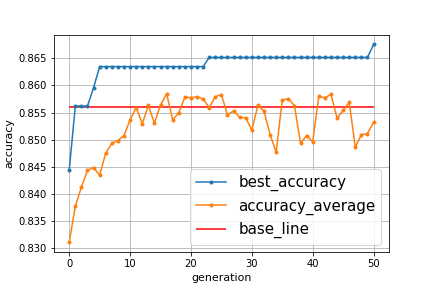
\includegraphics[scale=0.6]{graph.png}
	\caption{accuracyの推移\label{fig:graph}}
\end{figure}

また,base\_lineは0.8561であり,これはtraning\_dataを4000枚,epoch数30で10回学習させたときの平均値である.
前回より突然変異率を上げたため平均値が不安定である.
そして最終的な最良値は0.8676となった.
\ また,これで得られた染色体を50000枚のtraining\_dataに適用し,
100000枚のデータとしてepoch数30で学習させたところaccuracyは0.8832となった.\\
\ 次に,図\ref{fig:TransImg}に異なる上位3個体の変換例を示す.

\ よくかかっていたものとして,Brightness,shearY,Contrast,,Mirror,Posterizeがあげられる.
\section{今後の方針}
\ 今までは水増しについてoriginal画像に変換した画像を追加したものをひとつのdatasetとして実験を行っていたが,先行研究にあるようにBatchごとに適用する方法に変えた方がよいのではないかと思う.


\begin{figure*}[h]
	\begin{center}
		\centering
		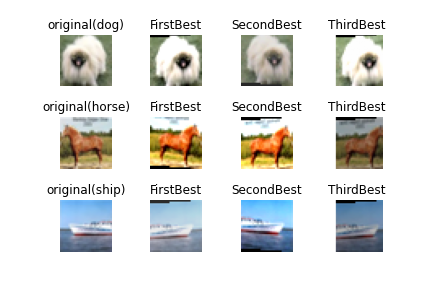
\includegraphics[scale=0.9]{fig.png}
		\caption{変換例\label{fig:TransImg}}
	\end{center}
\end{figure*}



\end{document}


